\section{Streaming video}
\label{sec:attend_the_course}

Through the platform of e-learning, the student will find their own course of interest selecting it from those available.
The user chosen and eventually paid the course,then he can start his training.

Also for streaming it has created a web component that allows the video vision, hiding all encountered problems and complexity resolved on the thesis work see(\ref{sec:HLS and VideoJS}).

\begin{lstlisting}[language=html]
  <deck-video src="{{lecture.video}}"></deck-video>
\end{lstlisting}

tale web component incapsula tutte le librerie e lo stile css necessari alla fruizione di un qualsiasi video in formto m3u8 che viene passato attraverso un url.

The final result will be a player to stream video content in qualsiasi web browser as you can see in the picture

\begin{figure}[htb]
 \centering
 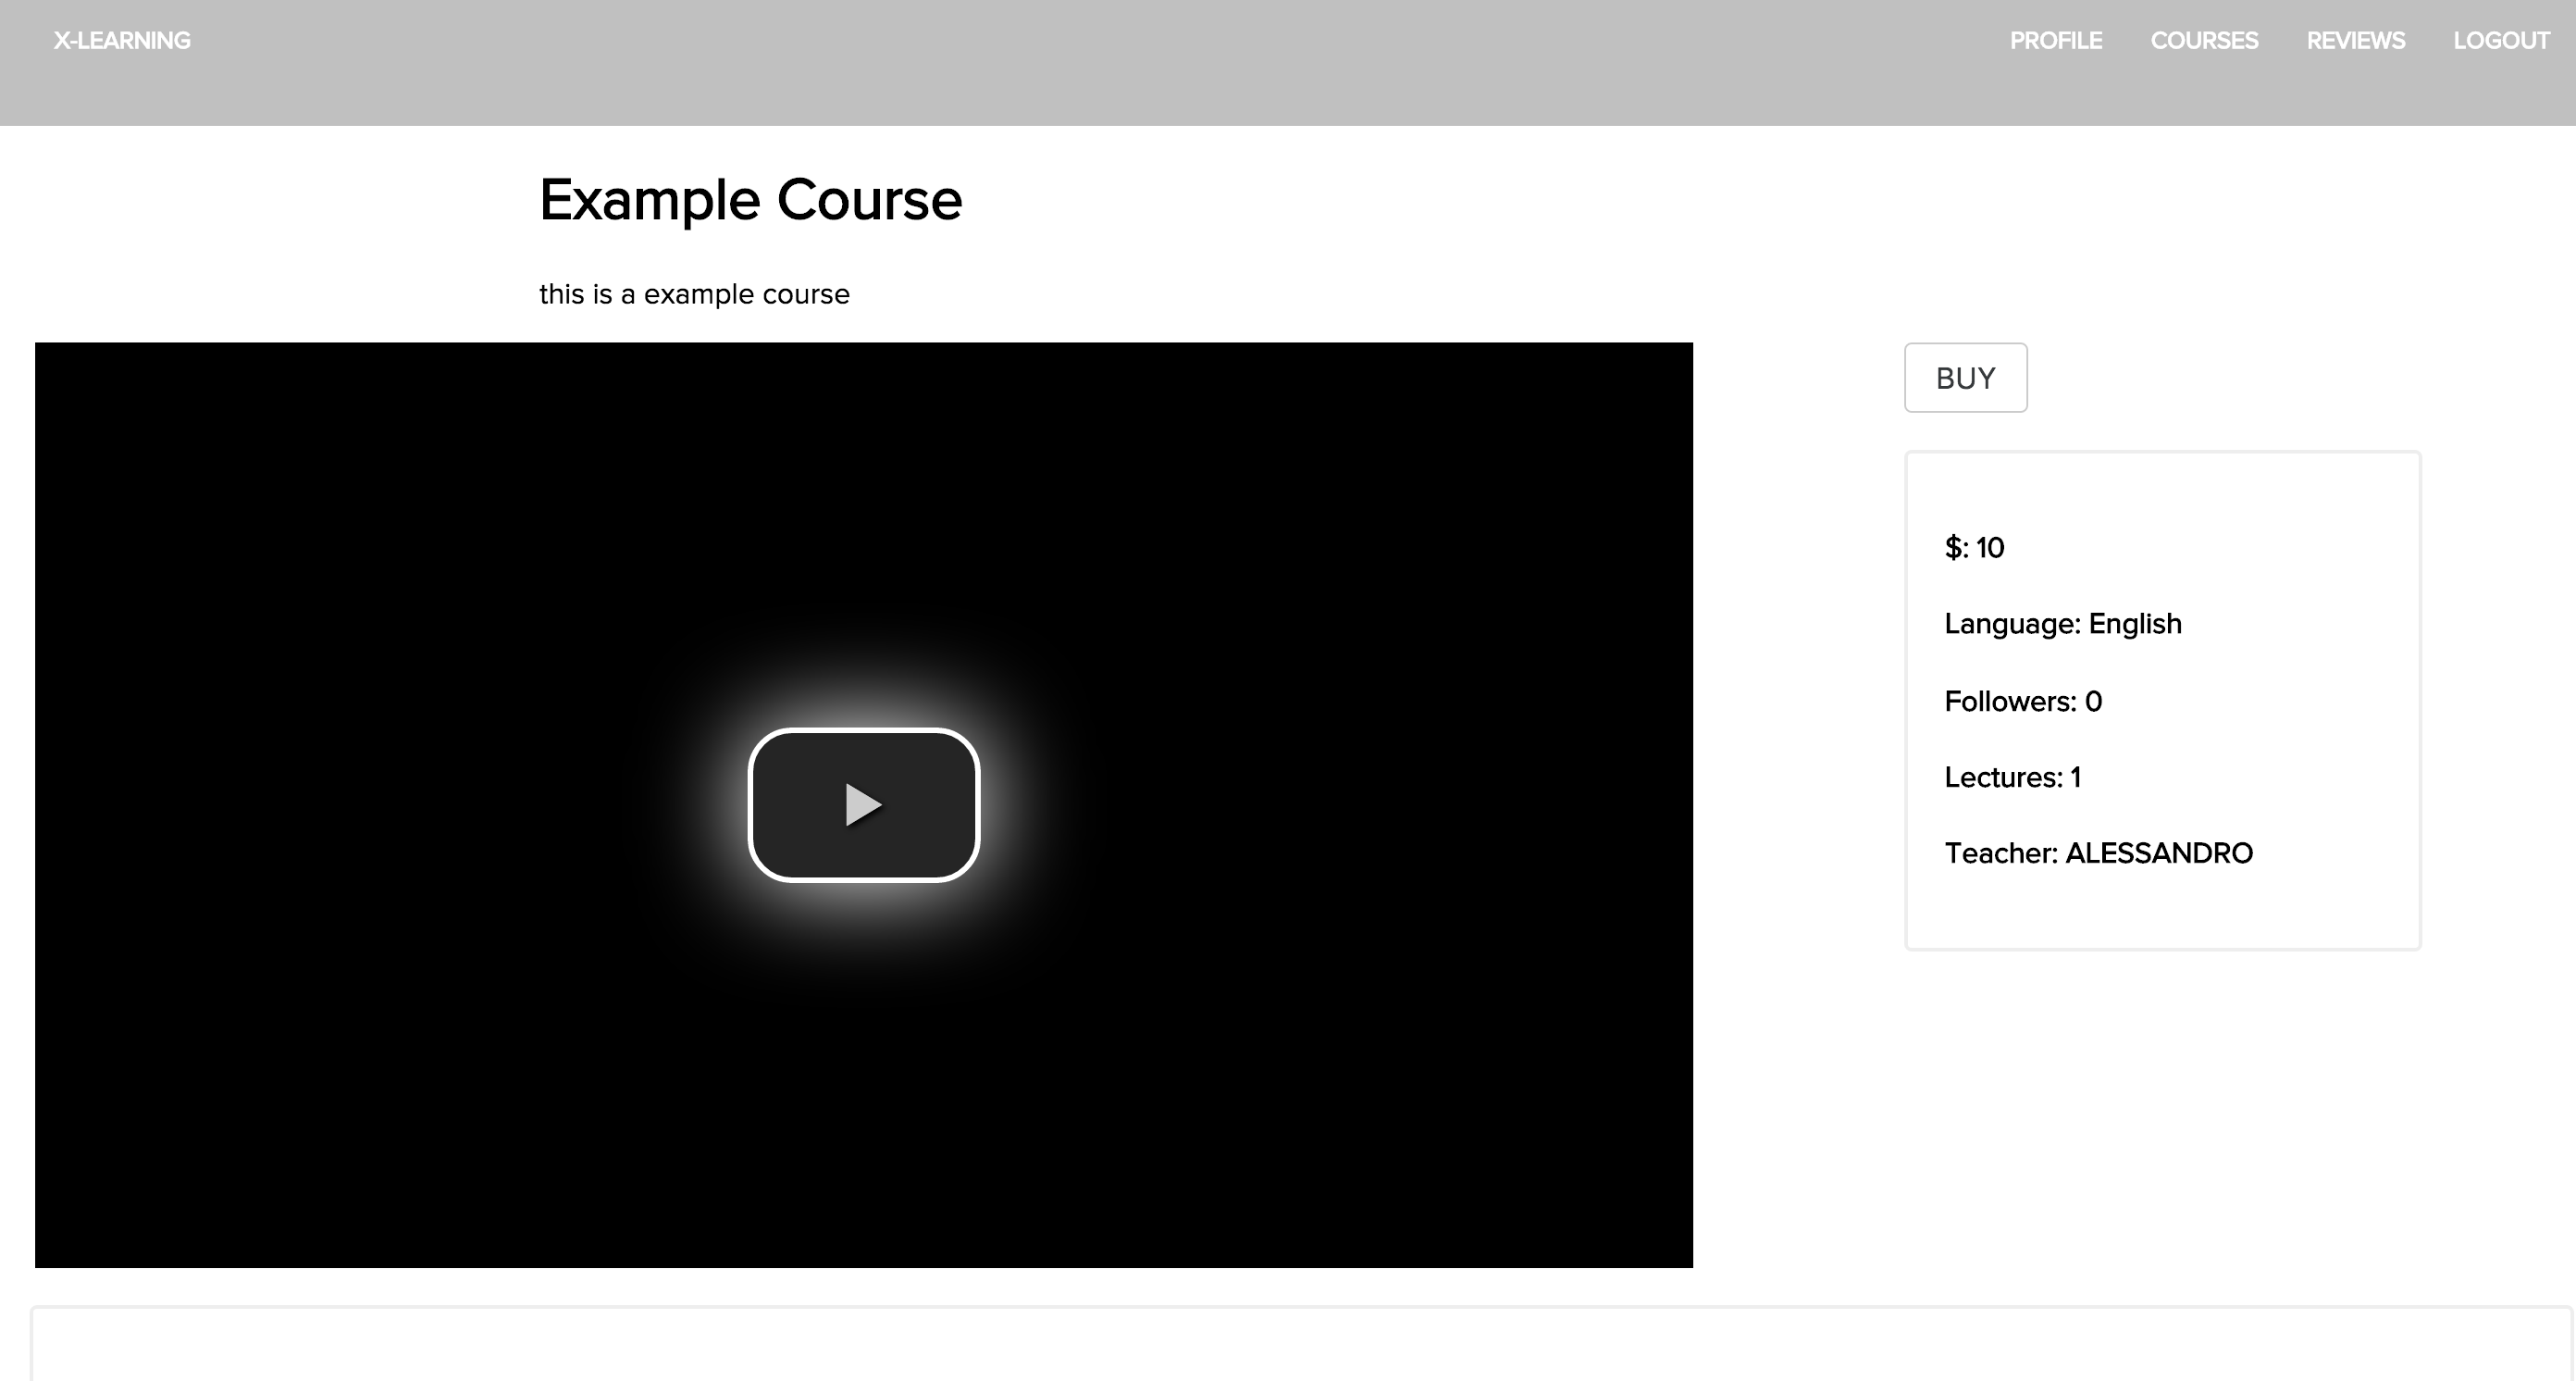
\includegraphics[width=1.0\linewidth]{images/chapter6/deck_video.png}\hfill
 \caption[Video player]{Video player}
 \label{fig:fourV}
\end{figure}
